\chapter{Mécanique hamiltonienne}\label{ch:b3:hamiltonian-mechanics}

Photographiez mille fois un pendule et portez, pour chaque cliché,
son angle en fonction de son moment cinétique~: les points se rangent sur
une courbe fermée, et tout mouvement possible du pendule est une telle
courbe --- \omterm{prop:b3:lagrangian-mechanics:modes}{petites oscillations} sur des ovales emboîtés, tours complets
sur des lignes ondulées au-dessus et au-dessous, et entre les deux une
unique courbe croisée qui sépare les deux régimes. Cette image, le
\emph{\omterm{def:b3:hamiltonian-mechanics:portrait}{portrait de phase}}, est le cœur de la reformulation que Hamilton
donna de la mécanique en 1833~: l'état d'un système est un point dans
l'espace des coordonnées \emph{et} des moments, son évolution est un
écoulement dans cet espace, et cet écoulement est engendré par une
seule fonction, l'énergie, à travers deux équations du premier ordre
d'une belle symétrie. Le gain n'est pas la facilité des calculs ---
Lagrange l'emporte le plus souvent --- mais la bonne
\emph{géométrie}~: l'écoulement conserve le volume dans l'\omterm{def:b3:hamiltonian-mechanics:hamiltonian}{espace des
phases}, ce qui fondera la physique statistique~; et son squelette
algébrique, le \omterm{def:b3:hamiltonian-mechanics:poisson}{crochet de Poisson}, est exactement ce que la mécanique
quantique promouvra en commutateur. Ce chapitre est la charnière entre
la mécanique des objets et la physique du vingtième siècle.

\section{De Lagrange à Hamilton}

\begin{definition}[Hamiltonien et équations canoniques]\label{def:b3:hamiltonian-mechanics:hamiltonian}
\index{hamiltonien}\index{équations canoniques}\index{espace des phases}
Pour un système de \omterm{def:b3:lagrangian-mechanics:action}{lagrangien} $L(q, \dot q, t)$, exprimons les vitesses
en fonction des moments $p_i = \partial L/\partial\dot q_i$ et
définissons le \emph{hamiltonien} comme la transformée de Legendre
\[
H(q, p, t) = \sum_i p_i\dot q_i - L ,
\]
fonction des coordonnées et des \emph{moments}. L'espace de dimension
$2n$ des $(q_1, \dots, q_n, p_1, \dots, p_n)$ est l'\emph{espace des
phases}~; un seul de ses points --- un \emph{état} --- détermine tout
l'avenir et tout le passé du système par les \emph{équations
canoniques} du
\cref{thm:b3:hamiltonian-mechanics:canonical}.
\end{definition}

\begin{theorem}[Équations de Hamilton]\label{thm:b3:hamiltonian-mechanics:canonical}
Les \omterm{thm:b3:lagrangian-mechanics:euler-lagrange}{équations d'Euler--Lagrange} équivalent aux $2n$ équations du
premier ordre
\[
\dot q_i = \frac{\partial H}{\partial p_i} , \qquad
\dot p_i = -\frac{\partial H}{\partial q_i} .
\]
\end{theorem}

\begin{proof}
Différentions $H = \sum p_i\dot q_i - L$ comme fonction de $(q, p, t)$~:
$\dd H = \sum(\dot q_i\,\dd p_i + p_i\,\dd\dot q_i) - \sum(
\partial_{q_i}L\,\dd q_i + \partial_{\dot q_i}L\,\dd\dot q_i) -
\partial_tL\,\dd t$. Les termes en $\dd\dot q_i$ se compensent par la
définition de $p_i$ --- tout l'intérêt de la transformée de Legendre ---
et il reste $\dd H = \sum(\dot q_i\,\dd p_i - \partial_{q_i}L\,\dd q_i) -
\partial_tL\,\dd t$. En lisant les dérivées partielles~:
$\partial H/\partial p_i = \dot q_i$ et $\partial H/\partial q_i =
-\partial L/\partial q_i$, qui vaut $-\dot p_i$ par Euler--Lagrange.
(Et aussi $\partial_tH = -\partial_tL$.)
\end{proof}

\begin{proposition}[Ce qu'est $H$]\label{prop:b3:hamiltonian-mechanics:energy}
$H$ coïncide avec la \omterm{prop:b3:lagrangian-mechanics:energy}{fonction énergie} $h$ du chapitre précédent~:
le long d'un mouvement, $\dd H/\dd t = \partial H/\partial t$, donc $H$
est conservé dès qu'il ne dépend pas explicitement du temps~; et
lorsque l'énergie cinétique est quadratique en les vitesses avec des
contraintes indépendantes du temps, $H = E_k + E_p$, l'énergie
mécanique --- écrite désormais dans les variables $(q, p)$.
\end{proposition}

\begin{proof}
$\dd H/\dd t = \sum(\partial_{q_i}H\,\dot q_i + \partial_{p_i}H\,\dot
p_i) + \partial_tH = \sum(\partial_{q_i}H\,\partial_{p_i}H -
\partial_{p_i}H\,\partial_{q_i}H) + \partial_tH = \partial_tH$~: la
symétrie des \omterm{def:b3:hamiltonian-mechanics:hamiltonian}{équations canoniques} annule identiquement la somme.
L'identification à $E_k + E_p$ est
\cref{prop:b3:lagrangian-mechanics:energy}.
\end{proof}

\begin{example}[Deux hamiltoniens]\label{ex:b3:hamiltonian-mechanics:examples}
Masse sur un ressort~: $p = m\dot x$, donc
\[
H = \frac{p^2}{2m} + \frac12 kx^2 ;
\]
les \omterm{def:b3:hamiltonian-mechanics:hamiltonian}{équations canoniques} $\dot x = p/m$, $\dot p = -kx$ sont la paire
familière. Pendule~: $p = m\ell^2\dot\theta$ et
\[
H = \frac{p^2}{2m\ell^2} - mg\ell\cos\theta .
\]
Dans les deux cas $H$ est l'énergie, constante sur chaque mouvement~:
les mouvements \emph{sont} les courbes de niveau de $H$ dans le plan $(q,p)$.
\end{example}

\begin{method}[La recette hamiltonienne]\label{met:b3:hamiltonian-mechanics:recipe}
(1) À partir de $L$, calculer les moments $p_i = \partial L/\partial\dot q_i$
et inverser pour les $\dot q_i$. (2) $H = \sum p_i\dot q_i - L$,
exprimé en $(q, p)$ seulement --- pour un système naturel, simplement
$E_k + E_p$ avec $E_k$ réécrite en les moments. (3) Écrire les
\omterm{def:b3:hamiltonian-mechanics:hamiltonian}{équations canoniques}. (4) Tracer les courbes de niveau de $H$~: pour un
degré de liberté ce sont les trajectoires, et tout le mouvement
qualitatif --- oscillations, rotations, équilibres, \omterm{def:b3:hamiltonian-mechanics:portrait}{séparatrices} --- se
lit sans rien résoudre.
\end{method}

\section{L'espace des phases}

\begin{definition}[Portrait de phase, points fixes, séparatrice]\label{def:b3:hamiltonian-mechanics:portrait}
\index{portrait de phase}\index{point fixe}\index{séparatrice}
Le \emph{portrait de phase} d'un système est la famille de ses
trajectoires dans l'\omterm{def:b3:hamiltonian-mechanics:hamiltonian}{espace des phases}. Un \emph{point fixe} est un état
où les deux \omterm{def:b3:hamiltonian-mechanics:hamiltonian}{équations canoniques} s'annulent --- un équilibre~: un
minimum du potentiel apparaît comme un \emph{centre} entouré de courbes
fermées, un maximum comme un \emph{col} par lequel passe une
\emph{séparatrice}, la trajectoire qui partage l'\omterm{def:b3:hamiltonian-mechanics:hamiltonian}{espace des phases} en
régions de mouvements qualitativement différents.
\end{definition}

\begin{example}[Le portrait de phase du pendule]\label{ex:b3:hamiltonian-mechanics:pendulum-portrait}
Pour $H = p^2/2m\ell^2 - mg\ell\cos\theta$~: des ovales fermés autour de
$(0, 0)$ --- les \emph{librations}, oscillations ordinaires~; des
courbes ondulées à $|p|$ grand --- les \emph{rotations}, le pendule
tournant par le haut~; et par les cols en $\theta = \pm\pi$ la
\omterm{def:b3:hamiltonian-mechanics:portrait}{séparatrice}, d'énergie $E = +mg\ell$, sur laquelle le pendule met un
temps infini à atteindre le sommet. Un état sur la \omterm{def:b3:hamiltonian-mechanics:portrait}{séparatrice} est
l'oscillation lancée \emph{exactement} assez fort pour arriver à la
position inversée sans la moindre marge.
\end{example}

\begin{omfigure}
\begin{tikzpicture}
  \begin{axis}[omaxis, axis x line=bottom, axis y line=left,
    width=11.6cm, height=6.4cm, xmin=-180, xmax=180, ymin=-3.2, ymax=3.2,
    xlabel={$\theta$ (degrés)},
    xlabel style={at={(axis description cs:0.5,-0.08)}, anchor=north},
    ylabel={$p$ (en unités de $m\ell^2\omega_0$)},
    xtick={-180,-90,0,90,180}, ytick={-2,0,2}, clip=false]
    % librations E/mgl = -0.5 and 0.4 : p = ±sqrt(2(E'+cos x)), E'=E/mgl
    \addplot[omDef, thick, domain=-60:60, samples=80] {sqrt(2*(-0.5+cos(x)))};
    \addplot[omDef, thick, domain=-60:60, samples=80] {-sqrt(2*(-0.5+cos(x)))};
    \addplot[omDef, thick, domain=-113.5:113.5, samples=100] {sqrt(2*(0.4+cos(x)))};
    \addplot[omDef, thick, domain=-113.5:113.5, samples=100] {-sqrt(2*(0.4+cos(x)))};
    % separatrix E'=1: p=±2cos(x/2)
    \addplot[omThm, very thick, domain=-180:180, samples=100] {2*cos(x/2)};
    \addplot[omThm, very thick, domain=-180:180, samples=100] {-2*cos(x/2)};
    % rotations E'=2 and 3.5
    \addplot[omExo, thick, domain=-180:180, samples=100] {sqrt(2*(2+cos(x)))};
    \addplot[omExo, thick, domain=-180:180, samples=100] {-sqrt(2*(2+cos(x)))};
    \addplot[omExo, thick, domain=-180:180, samples=100] {sqrt(2*(3.5+cos(x)))};
    \addplot[omExo, thick, domain=-180:180, samples=100] {-sqrt(2*(3.5+cos(x)))};
    % fixed points
    \fill (axis cs:0,0) circle (1.8pt);
    \fill (axis cs:180,0) circle (1.8pt);
    \fill (axis cs:-180,0) circle (1.8pt);
    % flow arrows
    \draw[->, thick] (axis cs:-6,1.66) -- (axis cs:6,1.66);
    \draw[->, thick] (axis cs:6,-1.66) -- (axis cs:-6,-1.66);
    \draw[->, thick] (axis cs:-6,2.45) -- (axis cs:6,2.45);
    \draw[->, thick] (axis cs:6,-2.45) -- (axis cs:-6,-2.45);
    \node[omDef, font=\scriptsize, anchor=west] at (axis cs:-52,0.5) {libration};
    \node[omThm, font=\scriptsize, anchor=west] at (axis cs:97,1.75) {séparatrice};
    \node[omExo, font=\scriptsize, anchor=west] at (axis cs:-172,2.93) {rotation};
  \end{axis}
\end{tikzpicture}

{\small Le \omterm{def:b3:hamiltonian-mechanics:portrait}{portrait de phase} du pendule~: les courbes de niveau de $H$.
Les ovales fermés (oscillations) tournent dans le sens horaire autour
du centre~; au-dessus et au-dessous de la \omterm{def:b3:hamiltonian-mechanics:portrait}{séparatrice}, le pendule
tourne. Les cols en $\pm 180^\circ$ sont l'équilibre inversé.}
\end{omfigure}

\begin{theorem}[Théorème de Liouville]\label{thm:b3:hamiltonian-mechanics:liouville}
\index{théorème de Liouville}
L'écoulement \omterm{def:b3:hamiltonian-mechanics:hamiltonian}{hamiltonien} conserve le volume dans l'\omterm{def:b3:hamiltonian-mechanics:hamiltonian}{espace des phases}~:
si une région d'états initiaux est entraînée par les \omterm{def:b3:hamiltonian-mechanics:hamiltonian}{équations
canoniques}, son volume (son aire, pour un degré de liberté) ne change
jamais --- quelle que soit la forme qu'elle prend.
\end{theorem}

\begin{proof}
L'écoulement dans l'\omterm{def:b3:hamiltonian-mechanics:hamiltonian}{espace des phases} a pour champ
de vitesse le couple $(\dot q_i, \dot p_i) = (\partial_{p_i}H,
-\partial_{q_i}H)$. Sa divergence vaut
\[
\sum_i\Big(\frac{\partial\dot q_i}{\partial q_i}
 + \frac{\partial\dot p_i}{\partial p_i}\Big)
 = \sum_i\Big(\frac{\partial^2H}{\partial q_i\partial p_i}
 - \frac{\partial^2H}{\partial p_i\partial q_i}\Big) = 0 :
\]
l'écoulement est incompressible, et un écoulement incompressible
transporte les volumes sans les changer, comme pour les fluides du
volume de deuxième année. (Le passage formel d'une divergence nulle à
la conservation du volume est le théorème de transport démontré là.)
\end{proof}

\begin{remark}[Pourquoi Liouville compte]\label{rem:b3:hamiltonian-mechanics:liouville-matters}
Rien dans la formulation de Newton ne suggère qu'une quelconque
grandeur soit incompressible. Dans l'image hamiltonienne c'est
automatique --- et c'est le permis de la physique statistique~: lorsque
nous décrivons un gaz de $10^{23}$ molécules par un nuage de points
dans l'\omterm{def:b3:hamiltonian-mechanics:hamiltonian}{espace des phases}, le \omterm{thm:b3:hamiltonian-mechanics:liouville}{théorème de Liouville} dit que le nuage
s'écoule comme un fluide incompressible, de sorte que le «~nombre
d'états dans un volume de l'\omterm{def:b3:hamiltonian-mechanics:hamiltonian}{espace des phases}~» est une grandeur que la
dynamique elle-même ne peut ni créer ni détruire. Le postulat
microcanonique de la physique statistique, plus loin dans ce volume,
repose exactement là-dessus.
\end{remark}

\begin{omfigure}
\begin{tikzpicture}[font=\small, >=Stealth]
  % free particle shear
  \begin{scope}
    \draw[->] (0,0) -- (5.2,0) node[right] {$q$};
    \draw[->] (0,0) -- (0,3.0) node[above] {$p$};
    \fill[omDef!30, draw=omDef, thick] (0.6,0.8) rectangle (1.6,2.2);
    \fill[omDef!30, draw=omDef, thick] (2.7,0.8) -- (3.7,0.8) -- (5.1,2.2) -- (4.1,2.2) -- cycle;
    \draw[->, thick] (1.85,1.5) -- (2.5,1.5);
    \node at (1.1,0.45) {$t = 0$};
    \node at (3.9,0.45) {$t > 0$};
  \end{scope}
  \node[font=\footnotesize] at (2.6,-0.7) {particule libre~: $\dot q = p/m$ cisaille la tache};
  % harmonic oscillator rotation
  \begin{scope}[xshift=9.6cm]
    \draw[->] (-2.6,0) -- (2.8,0) node[right] {$q$};
    \draw[->] (0,-1.55) -- (0,2.9) node[above] {$p$};
    \draw[gray, dashed] (0,0) circle (1.75);
    \fill[omThm!30, draw=omThm, thick] (1.35,0.35) -- (2.15,0.35) -- (2.15,0.95) -- (1.35,0.95) -- cycle;
    \begin{scope}[rotate=100]
    \fill[omThm!30, draw=omThm, thick] (1.35,0.35) -- (2.15,0.35) -- (2.15,0.95) -- (1.35,0.95) -- cycle;
    \end{scope}
    \draw[->, thick] (2.0,1.35) arc (35:75:2.35);
    \node at (2.5,-0.45) {$t = 0$};
    \node at (-1.15,2.45) {$t > 0$};
  \end{scope}
  \node[font=\footnotesize] at (9.6,-0.7) {oscillateur harmonique~: la tache tourne en bloc};
\end{tikzpicture}

{\small Le \omterm{thm:b3:hamiltonian-mechanics:liouville}{théorème de Liouville}~: l'écoulement déforme une région
d'états initiaux --- il la cisaille, il la fait tourner --- mais son
aire est exactement conservée.}
\end{omfigure}

\section{Crochets de Poisson}

\begin{definition}[Crochet de Poisson]\label{def:b3:hamiltonian-mechanics:poisson}
\index{crochet de Poisson}
Le \emph{crochet de Poisson} de deux fonctions $f(q, p, t)$ et
$g(q, p, t)$ sur l'\omterm{def:b3:hamiltonian-mechanics:hamiltonian}{espace des phases} est
\[
\{f, g\} = \sum_i\Big(
 \frac{\partial f}{\partial q_i}\frac{\partial g}{\partial p_i}
 - \frac{\partial f}{\partial p_i}\frac{\partial g}{\partial q_i}\Big) .
\]
Il est antisymétrique, linéaire en chaque argument, vérifie la règle du
produit $\{f, gh\} = \{f, g\}h + g\{f, h\}$, et satisfait pour les
coordonnées elles-mêmes les \emph{relations canoniques}
\[
\{q_i, p_j\} = \delta_{ij} , \qquad
\{q_i, q_j\} = \{p_i, p_j\} = 0 .
\]
\end{definition}

\begin{theorem}[L'évolution comme crochet]\label{thm:b3:hamiltonian-mechanics:evolution}
Le long de tout mouvement,
\[
\frac{\dd f}{\dd t} = \{f, H\} + \frac{\partial f}{\partial t} .
\]
En particulier, une grandeur sans dépendance explicite en temps est
conservée si et seulement si son crochet avec le \omterm{def:b3:hamiltonian-mechanics:hamiltonian}{hamiltonien} est nul~;
et les \omterm{def:b3:hamiltonian-mechanics:hamiltonian}{équations canoniques} elles-mêmes s'écrivent $\dot q_i = \{q_i, H\}$, $\dot p_i
= \{p_i, H\}$~: le \omterm{def:b3:hamiltonian-mechanics:hamiltonian}{hamiltonien} \emph{engendre} l'évolution temporelle.
\end{theorem}

\begin{proof}
Règle de dérivation composée et \omterm{def:b3:hamiltonian-mechanics:hamiltonian}{équations canoniques}~: $\dd f/\dd t = \sum(
\partial_{q_i}f\,\dot q_i + \partial_{p_i}f\,\dot p_i) + \partial_tf =
\sum(\partial_{q_i}f\,\partial_{p_i}H - \partial_{p_i}f\,
\partial_{q_i}H) + \partial_tf$.
\end{proof}

\begin{example}[Crochets du moment cinétique]\label{ex:b3:hamiltonian-mechanics:brackets}
Pour une particule, $L_z = xp_y - yp_x$ et ses compagnes par
permutation circulaire. Un calcul direct à partir des relations
canoniques donne
\[
\{L_x, L_y\} = L_z , \qquad
\{L_y, L_z\} = L_x , \qquad
\{L_z, L_x\} = L_y ,
\]
et $\{L^2, L_z\} = 0$~: les composantes du moment cinétique ne
«~commutent~» pas entre elles, mais chacune commute avec le carré
total. Retenez la forme de ces relations --- elles reviendront
textuellement, comme commutateurs, en mécanique quantique, où elles
dictent tout de la structure atomique.
\end{example}

\begin{remark}[La porte de la mécanique quantique]\label{rem:b3:hamiltonian-mechanics:doorway}
Dirac observa en 1925 que toute la mécanique quantique s'obtient en
gardant l'algèbre de la mécanique hamiltonienne et en remplaçant le
\omterm{def:b3:hamiltonian-mechanics:poisson}{crochet de Poisson} par le commutateur des opérateurs divisé par
$\iu\hbar$~: $\{q, p\} = 1$ devient $[\hat x, \hat p] = \iu\hbar$, la
conservation reste «~crochet avec $H$ nul~», et l'évolution temporelle
reste engendrée par le \omterm{def:b3:hamiltonian-mechanics:hamiltonian}{hamiltonien}. La théorie classique porte, dans
ses os, le squelette de la théorie quantique~; les chapitres de
mécanique quantique rendront cette correspondance explicite.
\end{remark}

\section{Action et invariants adiabatiques}

\begin{definition}[Variable d'action]\label{def:b3:hamiltonian-mechanics:action-variable}
\index{variable d'action}
Pour un système à un degré de liberté oscillant sur une trajectoire de
phase fermée, la \emph{variable d'\omterm{def:b3:lagrangian-mechanics:action}{action}} est l'aire enclose divisée
par $2\pi$~:
\[
I = \frac{1}{2\pi}\oint p\,\dd q .
\]
\end{definition}

\begin{proposition}[Action de l'oscillateur harmonique]\label{prop:b3:hamiltonian-mechanics:sho-action}
Pour $H = p^2/2m + \tfrac12 m\omega^2q^2$ à l'énergie $E$, la
trajectoire est une ellipse de demi-axes $\sqrt{2E/m\omega^2}$ et
$\sqrt{2mE}$, d'aire $2\pi E/\omega$~: d'où
\[
I = \frac{E}{\omega} , \qquad E = \omega I ,
\]
et la fréquence d'oscillation vaut $\partial E/\partial I = \omega$,
comme il se doit.
\end{proposition}

\begin{proof}
Aire d'une ellipse, $\pi ab = \pi\sqrt{2E/m\omega^2}\sqrt{2mE} =
2\pi E/\omega$.
\end{proof}

\begin{proposition}[Invariance adiabatique]\label{prop:b3:hamiltonian-mechanics:adiabatic}
\index{invariant adiabatique}
Si l'on fait varier \emph{lentement} un paramètre du système (une
longueur, une raideur, un champ) --- sur de nombreuses périodes
d'oscillation ---, l'énergie change, la fréquence change, mais
l'\omterm{def:b3:lagrangian-mechanics:action}{action} $I$ reste constante à une excellente approximation~: $I$ est
un \emph{\omterm{prop:b3:hamiltonian-mechanics:adiabatic}{invariant adiabatique}}. Pour l'oscillateur lentement modifié,
$E/\omega$ est donc conservé~: raidir lentement le ressort pour
doubler $\omega$ et l'énergie double avec lui.
\end{proposition}

\begin{proof}[Démonstration partielle]
Pour l'oscillateur de $\omega(t)$ lentement variable~: sur une période,
le travail fourni par le paramètre changeant se calcule par moyenne~;
le calcul (guidé dans \cref{exo:b3:hamiltonian-mechanics:11}) donne
$\dot E/E = \dot\omega/\omega$, c'est-à-dire $\dd(E/\omega)/\dd t = 0$
à l'ordre dominant. L'énoncé général, pour tout système oscillant
lentement déformé, est admis --- c'est la raison pour laquelle les
orbites planétaires survivent aux perturbations lentes, et le point de
départ de l'«~ancienne théorie des quanta~» ci-dessous.
\end{proof}

\begin{omfigure}
\begin{tikzpicture}[font=\small, >=Stealth]
  \begin{scope}
    \draw[->] (-2.9,0) -- (2.9,0) node[right] {$q$};
    \draw[->] (0,-1.9) -- (0,2.3) node[above] {$p$};
    \draw[omDef, thick] (0,0) ellipse (2.3 and 0.85);
    \draw[omThm, thick] (0,0) ellipse (1.63 and 1.2);
    \node[omDef, anchor=west] at (1.5,-1.1) {$\omega$};
    \node[omThm, anchor=west] at (0.2,1.45) {$2\omega$};
  \end{scope}
  \node[align=center] at (0,-2.75) {oscillateur lentement raidi~:\\l'ellipse se resserre, l'aire survit};
  \begin{scope}[xshift=8.2cm]
    \fill (0,2.1) circle (1.5pt);
    \draw[thick] (-1.1,2.1) -- (1.1,2.1);
    \foreach \i in {-0.95,-0.6,-0.25,0.1,0.45,0.8} \draw (\i,2.1) -- (\i+0.16,2.24);
    \draw[thick] (0,2.1) -- ++(-115:1.15) coordinate (bob1);
    \fill[omDef] (bob1) circle (2.6pt);
    \draw[dashed] (0,2.1) -- ++(-115:2.3) coordinate (bob2);
    \fill[omDef!45] (bob2) circle (2.6pt);
    \draw[->] (0.02,1.0) -- (0.02,1.6);
    \node[anchor=west] at (0.1,1.28) {on tire};
    \node[align=center] at (0,-0.85) {on raccourcit lentement un pendule qui oscille~:\\$E/\omega$ constant, l'amplitude croît};
  \end{scope}
\end{tikzpicture}

{\small Invariance adiabatique. À gauche~: lorsque $\omega$ est
lentement doublée, l'ellipse de phase change de forme à aire constante,
donc $E = \omega I$ double. À droite~: hisser le fil d'un pendule qui
oscille lui injecte de l'énergie exactement dans la proportion qui
maintient $I = E/\omega$ fixe.}
\end{omfigure}

\begin{remark}[L'ancienne théorie des quanta]\label{rem:b3:hamiltonian-mechanics:old-quantum}
Pourquoi les atomes ont-ils des énergies discrètes~? La première
réponse quantitative (Bohr 1913, Sommerfeld 1915) fut écrite dans la
langue de ce chapitre~: parmi tous les mouvements classiques, la nature
garde ceux dont l'intégrale d'\omterm{def:b3:lagrangian-mechanics:action}{action} est un nombre entier de constantes
de Planck,
\[
\oint p\,\dd q = nh .
\]
Appliquée à l'oscillateur harmonique, elle donne $E_n = n\hbar\omega$
(il n'y manque que la moitié du vrai $\big(n + \tfrac12\big)\hbar
\omega$)~; appliquée à une particule dans une boîte elle donne
\emph{exactement} les niveaux du volume de deuxième année~; appliquée à
l'atome d'hydrogène (\cref{pb:b3:hamiltonian-mechanics:1}) elle donne
le spectre mesuré à quatre chiffres. La règle était quantitativement
juste et conceptuellement provisoire --- et, l'\omterm{def:b3:lagrangian-mechanics:action}{action} étant un
\omterm{prop:b3:hamiltonian-mechanics:adiabatic}{invariant adiabatique}, le nombre quantique $n$ ne change pas sous les
perturbations lentes, ce qui explique qu'une telle règle ait pu
fonctionner. La vraie théorie commence cinq chapitres plus loin.
\end{remark}

\begin{omfigure}
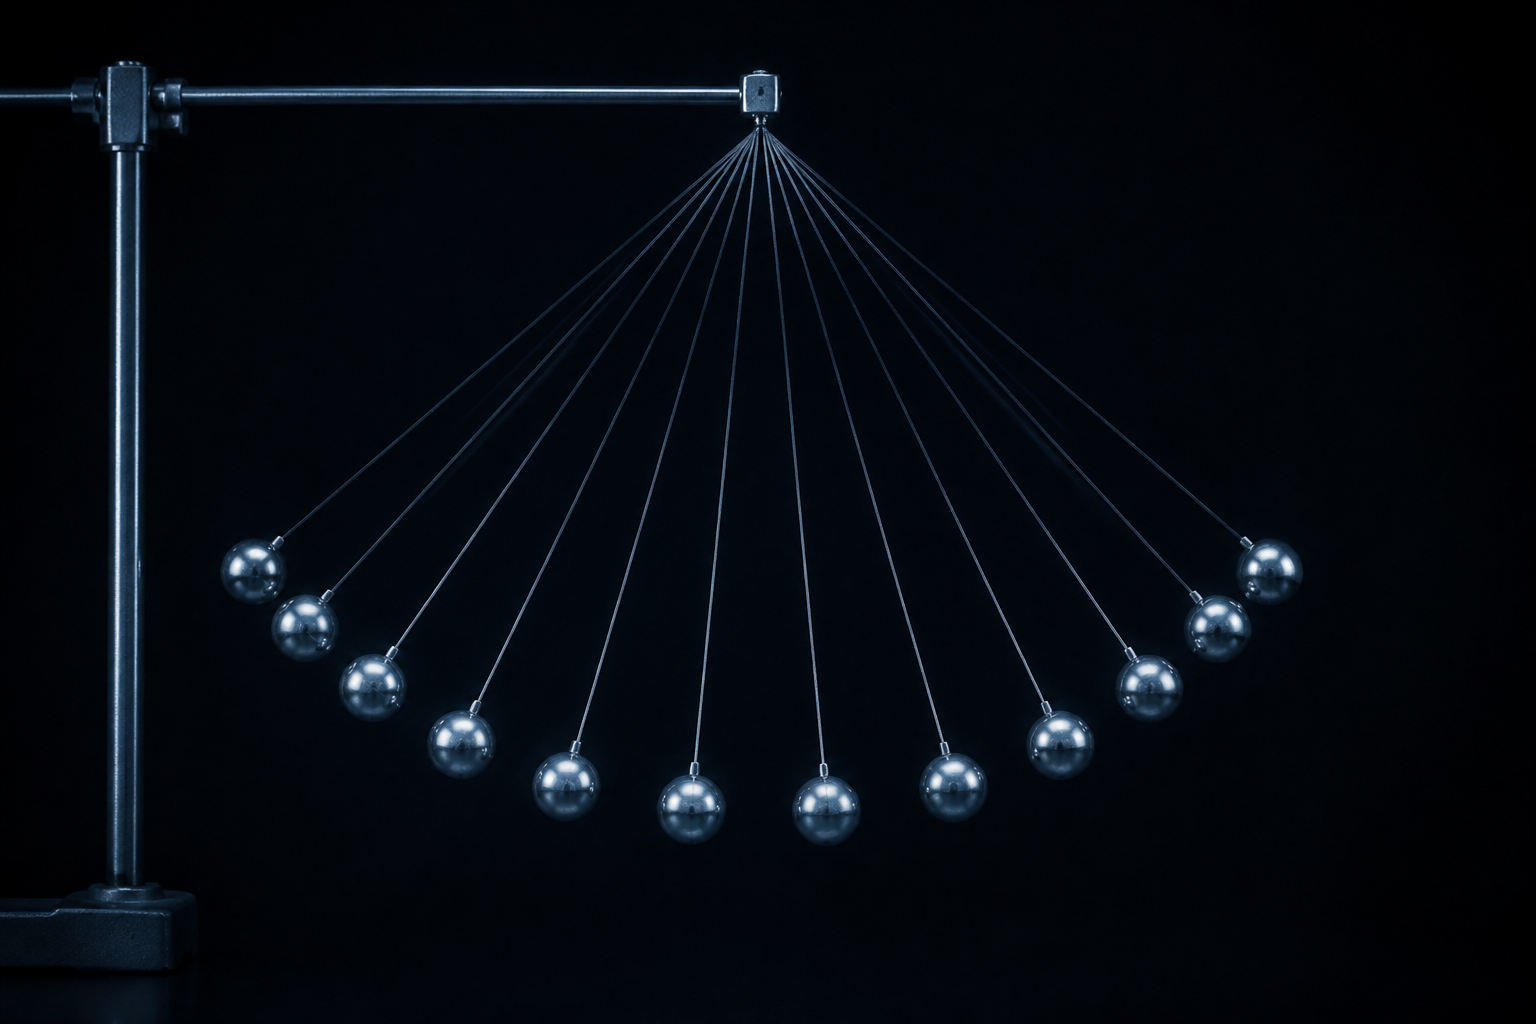
\includegraphics[width=0.58\linewidth]{images/book5/ai/b5-02-pendulum-strobe.png}

{\small Un pendule photographié au stroboscope~: les positions se pressent près des points de rebroussement, où la masse s'attarde, et s'espacent en bas, où elle se hâte --- une photographie du \omterm{def:b3:hamiltonian-mechanics:portrait}{portrait de phase} que ce chapitre trace avec des équations.}
\end{omfigure}

\section{Exercices}

\begin{exercise}[$\star$]\label{exo:b3:hamiltonian-mechanics:1}
Pour la masse sur un ressort~: (a) construire $H$ à partir de $L$ et vérifier que $H =
E_k + E_p$~; (b) écrire les \omterm{def:b3:hamiltonian-mechanics:hamiltonian}{équations canoniques} et vérifier qu'elles
redonnent $\ddot x = -\omega^2x$~; (c) montrer que les trajectoires
sont des ellipses dans le plan $(x, p)$ et donner leurs demi-axes à
l'énergie $E$~; (d) en quel sens le point représentatif tourne-t-il~?
\end{exercise}

\begin{exercise}[$\star$]\label{exo:b3:hamiltonian-mechanics:2}
La perle sur le cerceau tournant du chapitre précédent a pour $L =
\tfrac12 mR^2\dot\theta^2 + \tfrac12 m\omega^2R^2\sin^2\theta +
mgR\cos\theta$. (a) Calculer $p$ et $H$. (b) $H$ est-il conservé~?
Est-ce l'énergie mécanique~? (c) Tracer les courbes de niveau de $H$
pour $\omega^2 < g/R$ et $\omega^2 > g/R$, à l'aide du potentiel
effectif de ce chapitre. (d) Identifier les centres, les cols et les
\omterm{def:b3:hamiltonian-mechanics:portrait}{séparatrices} dans le cas rapide.
\end{exercise}

\begin{exercise}[$\star$]\label{exo:b3:hamiltonian-mechanics:3}
Une balle rebondit élastiquement sur le sol, $H = p^2/2m + mgz$ ($z >
0$). (a) Tracer la trajectoire de phase d'un vol, puis du mouvement de
rebond entier. (b) Que fait le rebond élastique au point
représentatif~? (c) Calculer l'aire enclose pour une hauteur maximale
$z_{\max}$, ainsi que l'\omterm{def:b3:lagrangian-mechanics:action}{action} $I$. (d) La règle de Bohr--Sommerfeld
$\oint p\,\dd z = nh$ appliquée à un neutron rebondissant ($m =
\qty{1.67e-27}{kg}$) donne des hauteurs de rebond quantifiées~: estimer
la plus basse et comparer aux \qty{15}{\micro m} mesurés dans
l'expérience d'états quantiques gravitationnels de 2002.
\end{exercise}

\begin{exercise}[$\star$]\label{exo:b3:hamiltonian-mechanics:4}
À partir des seules relations canoniques, calculer (a) $\{x^2, p\}$~;
(b) $\{xp, H\}$ pour $H = p^2/2m + E_p(x)$, et interpréter les deux
termes (ce crochet gouverne le \emph{théorème du viriel})~; (c)
$\{L_z, x\}$ et $\{L_z, p_x\}$~; (d) montrer que si $\{f, H\} = 0$ et
$\{g, H\} = 0$ alors $\{f, g\}$ est aussi conservé (utiliser
l'identité de Jacobi, admise~:
$\{f,\{g,h\}\} + \{g,\{h,f\}\} + \{h,\{f,g\}\} = 0$).
\end{exercise}

\begin{exercise}[$\star\star$]\label{exo:b3:hamiltonian-mechanics:5}
Le pendule au voisinage de sa \omterm{def:b3:hamiltonian-mechanics:portrait}{séparatrice}. (a) Donner l'énergie de la
\omterm{def:b3:hamiltonian-mechanics:portrait}{séparatrice} et le $|p|$ maximal sur celle-ci. (b) Montrer que sur la \omterm{def:b3:hamiltonian-mechanics:portrait}{séparatrice} $p =
\pm 2m\ell^2\omega_0\cos(\theta/2)$ avec $\omega_0 = \sqrt{g/\ell}$.
(c) À l'aide de $\dot\theta = p/m\ell^2$, montrer que le temps pour
aller de $\theta$ au sommet diverge logarithmiquement. (d) Un pendule
réel lâché juste au-dessous de la \omterm{def:b3:hamiltonian-mechanics:portrait}{séparatrice} reste un long moment près
de la position inversée avant de repartir --- relier cela à (c), et au
ralentissement observé près de tout col.
\end{exercise}

\begin{exercise}[$\star\star$]\label{exo:b3:hamiltonian-mechanics:6}
Une particule chargée dans un champ magnétique a pour $H = (\vect p -
q\vect A)^2/2m$, où $\vect p$ est le \omterm{def:b3:lagrangian-mechanics:momentum}{moment conjugué} du chapitre
précédent. (a) Écrire les \omterm{def:b3:hamiltonian-mechanics:hamiltonian}{équations canoniques} pour $\vect A = \tfrac12
B(-y, x, 0)$ et vérifier qu'elles donnent le mouvement cyclotron. (b) Montrer que $H =
\tfrac12 m\vect v^{\,2}$~: le champ magnétique ne travaille pas. (c)
Calculer le crochet des deux grandeurs conservées $\pi_x = p_x - \tfrac12
qBy$ et $\pi_y = p_y + \tfrac12 qBx$ (vérifier d'abord que chacune est
conservée), et montrer que $\{\pi_x, \pi_y\} = -qB$~: deux grandeurs
conservées dont le crochet est une constante. (d) Utiliser
\cref{exo:b3:hamiltonian-mechanics:4}(d) pour expliquer pourquoi
aucune troisième grandeur conservée indépendante n'était à en attendre.
\end{exercise}

\begin{exercise}[$\star\star$]\label{exo:b3:hamiltonian-mechanics:7}
Liouville à la main. (a) Pour la particule libre, l'écoulement est $q \to q +
pt/m$, $p \to p$~: montrer qu'un rectangle devient un parallélogramme
de même aire. (b) Pour l'oscillateur harmonique, montrer que
l'écoulement est une rotation (en unités convenables) et conclure. (c)
Pour l'oscillateur \emph{amorti} $\ddot x = -\omega^2x - \gamma\dot x$,
écrire la divergence de l'écoulement dans le plan $(x, v)$ et montrer
que les aires décroissent comme $\eu^{-\gamma t}$~: l'amortissement
n'est pas \omterm{def:b3:hamiltonian-mechanics:hamiltonian}{hamiltonien}. (d) Où passe physiquement l'aire perdue~?
\end{exercise}

\begin{exercise}[$\star\star$]\label{exo:b3:hamiltonian-mechanics:8}
Mouvement plan dans un potentiel central, $H = (p_r^2 + p_\varphi^2/r^2)/2m
+ E_p(r)$. (a) Écrire les quatre \omterm{def:b3:hamiltonian-mechanics:hamiltonian}{équations canoniques}. (b) Montrer que $\{
p_\varphi, H\} = 0$ et identifier la loi de conservation. (c) Ramener à
un \omterm{def:b3:hamiltonian-mechanics:hamiltonian}{hamiltonien} radial à une dimension avec un potentiel effectif. (d)
Pour $E_p = -k/r$, situer l'orbite circulaire à $p_\varphi$ donné et
donner son énergie --- à quantifier dans
\cref{pb:b3:hamiltonian-mechanics:1}.
\end{exercise}

\begin{exercise}[$\star\star$]\label{exo:b3:hamiltonian-mechanics:9}
(a) Vérifier $\{L_x, L_y\} = L_z$ à partir des relations canoniques.
(b) En déduire les deux autres crochets par permutation circulaire.
(c) Montrer que $\{L^2, L_z\} = 0$. (d) Un solide tourne librement~: en prenant $H =
L^2/2J$ (inertie à symétrie sphérique), montrer que les trois $L_i$
sont conservés~; qu'en est-il d'un solide à moments d'inertie inégaux
(répondre qualitativement à partir des crochets)~?
\end{exercise}

\begin{exercise}[$\star\star\star$]\label{exo:b3:hamiltonian-mechanics:10}
Niveaux de l'ancienne théorie des quanta. (a) Montrer que
$\oint p\,\dd q = nh$ appliquée à l'oscillateur harmonique donne
$E_n = n\hbar\omega$, à l'aide de
\cref{prop:b3:hamiltonian-mechanics:sho-action}. (b) L'appliquer à la
particule dans une boîte de longueur $a$ et retrouver exactement $E_n =
n^2h^2/8ma^2$. (c) Pour une molécule diatomique modélisée par un
oscillateur de raideur $k = \qty{1.9e3}{N/m}$ et de masse réduite $\qty{1.14e-26}
{kg}$ (monoxyde de carbone), calculer $\hbar\omega$ en eV et la
longueur d'onde de l'émission $n = 1 \to 0$~; dans quel domaine
spectral tombe-t-elle~? (d) Les vrais niveaux valent
$(n + \tfrac12)\hbar\omega$~: la moitié manquante change-t-elle les
longueurs d'onde \emph{émises}~? Quelle expérience détecte, elle, cette
demi-quantité de point zéro~?
\end{exercise}

\begin{exercise}[$\star\star\star$]\label{exo:b3:hamiltonian-mechanics:11}
Invariance adiabatique de $E/\omega$, démontrée. Une masse sur un
ressort dont la raideur $k(t)$ croît lentement. (a) Montrer que $\dot E = \tfrac12\dot k\,
x^2$ le long du mouvement exact. (b) Moyenner sur une période à $k$ fixée~:
à l'aide de $\langle\tfrac12 kx^2\rangle = E/2$, montrer que $\langle\dot E\rangle
= \dot k\,E/2k$. (c) Conclure $\dd\ln E = \tfrac12\dd\ln k = \dd\ln
\omega$, d'où $E/\omega$ constant. (d) Un pendule oscillant avec
l'amplitude $\theta_0 = 5^\circ$ voit son fil lentement raccourci de
\qty{1.0}{m} à \qty{0.5}{m}~: trouver la nouvelle amplitude et le
facteur de croissance de son énergie, et dites d'où vient cette énergie.
\end{exercise}

\begin{exercise}[$\star\star\star$]\label{exo:b3:hamiltonian-mechanics:12}
L'aire intérieure à la \omterm{def:b3:hamiltonian-mechanics:portrait}{séparatrice} du pendule est un nombre d'états
quantiques. (a) Montrer que $\oint p\,\dd\theta$ le long de la
\omterm{def:b3:hamiltonian-mechanics:portrait}{séparatrice} vaut $16m\ell^2\omega_0$. (b) Par la règle de
Bohr--Sommerfeld, le nombre d'états quantiques d'énergie inférieure à celle de la \omterm{def:b3:hamiltonian-mechanics:portrait}{séparatrice} vaut $N \approx
16m\ell^2\omega_0/h$~: l'évaluer pour une masse d'un gramme au bout
d'un fil de \qty{10}{cm}. (c) L'évaluer pour un oscillateur
moléculaire du genre de l'ammoniac~: $m \sim \qty{1e-26}{kg}$,
$\ell \sim \qty{1e-10}{m}$, $\omega_0 \sim \qty{1e14}{rad/s}$. (d)
Conclure~: où passe la frontière entre la mécanique qui a besoin de
$\hbar$ et celle qui n'en a pas besoin~?
\end{exercise}

\section{Problème~: l'ancienne théorie des quanta et l'hydrogène}

\begin{problem}[{Problème du week-end --- quantifier l'espace des
phases, peser le Rydberg}]\label{pb:b3:hamiltonian-mechanics:1}
En 1913 Bohr calcula le spectre de l'hydrogène à partir de la mécanique
planétaire et d'une seule règle quantique~; Sommerfeld reconnut dans
cette règle un énoncé sur l'aire dans l'\omterm{def:b3:hamiltonian-mechanics:hamiltonian}{espace des phases}. Ce problème
refait leur calcul avec les outils de ce chapitre. Données~: $m_{\text{e}} =
\qty{9.11e-31}{kg}$, $e = \qty{1.60e-19}{C}$, $1/4\pi\varepsilon_0 =
\qty{8.99e9}{N.m^2/C^2}$, $h = \qty{6.63e-34}{J.s}$, $c =
\qty{3.00e8}{m/s}$. On pose $k = e^2/4\pi\varepsilon_0$.

\medskip\noindent\textbf{Partie I --- Le \omterm{def:b3:hamiltonian-mechanics:hamiltonian}{hamiltonien} de Kepler.}
Un électron se déplace dans le plan autour d'un proton fixe.
\begin{enumerate}
  \item Justifier que l'on traite le proton comme fixe (rapport des masses), et écrire
        le \omterm{def:b3:hamiltonian-mechanics:hamiltonian}{hamiltonien} $H = \dfrac{p_r^2}{2m_{\text{e}}} +
        \dfrac{p_\varphi^2}{2m_{\text{e}}r^2} - \dfrac{k}{r}$.
  \item Écrire les quatre \omterm{def:b3:hamiltonian-mechanics:hamiltonian}{équations canoniques}.
  \item Montrer que $p_\varphi$ est conservé et le nommer.
  \item Ramener le mouvement radial au potentiel effectif
        $U_{\text{eff}}(r) = p_\varphi^2/2m_{\text{e}}r^2 - k/r$ et
        le tracer.
  \item Situer l'orbite circulaire~: $r_{\text{c}} =
        p_\varphi^2/m_{\text{e}}k$.
  \item Montrer que son énergie vaut $E = -k/2r_{\text{c}} =
        -m_{\text{e}}k^2/2p_\varphi^2$, et vérifier que c'est la moitié
        de l'énergie potentielle (le rapport du viriel des orbites
        gravitationnelles du volume de première année).
\end{enumerate}

\medskip\noindent\textbf{Partie II --- L'orbite classique.}
\begin{enumerate}[resume]
  \item Pour une orbite circulaire de rayon $r$, trouver la vitesse $v$
        et la fréquence orbitale $f_{\text{orb}}$ en fonction de $r$.
  \item Pour une orbite de taille atomique, $r = \qty{0.05}{nm}$~:
        calculer $v$ (et $v/c$), $f_{\text{orb}}$, et l'énergie en eV.
  \item Calculer le moment cinétique $p_\varphi$ de cette orbite et
        le comparer à $\hbar = h/2\pi$~: que suggère cette proximité~?
  \item Classiquement, un électron en orbite est un dipôle oscillant et
        rayonne (volume de deuxième année) à $f_{\text{orb}}$~; son
        énergie décroît en \qty{1e-11}{s} environ. Énoncer les deux
        prédictions fatales que cela donne pour les atomes, et ce que
        l'on observe à la place.
  \item Quel trait des spectres observés (raies discrètes, règle de
        combinaison $1/\lambda = R_H(1/n^2 - 1/n'^2)$) suggérait des
        \emph{niveaux} d'énergie discrets~?
  \item Expliquer pourquoi un \emph{\omterm{prop:b3:hamiltonian-mechanics:adiabatic}{invariant adiabatique}} est le
        candidat naturel pour une grandeur prenant des valeurs
        universelles fixées
        (rappeler \cref{prop:b3:hamiltonian-mechanics:adiabatic}).
\end{enumerate}

\medskip\noindent\textbf{Partie III --- La quantification.}
Imposons la règle de Sommerfeld au mouvement angulaire de l'orbite
circulaire~: $\oint p_\varphi\,\dd\varphi = nh$, $n = 1, 2, 3, \dots$
\begin{enumerate}[resume]
  \item Montrer que la règle s'écrit $p_\varphi = n\hbar$.
  \item En déduire les rayons permis $r_n = n^2a_0$ avec $a_0 =
        \hbar^2/m_{\text{e}}k$, et calculer $a_0$.
  \item En déduire les énergies permises $E_n = -E_{\text{I}}/n^2$
        avec $E_{\text{I}} = m_{\text{e}}k^2/2\hbar^2$, et calculer
        $E_{\text{I}}$ en joules et en eV.
  \item Calculer la vitesse sur la première orbite et vérifier que $v_1/c =
        k/\hbar c \approx 1/137$ (la constante de structure fine).
  \item Un photon emporte l'énergie d'une transition~: obtenir la
        formule de Rydberg et la valeur de $R_H = E_{\text{I}}/hc$~;
        comparer à la valeur mesurée \qty{1.097e7}{m^{-1}}.
  \item Calculer les longueurs d'onde des transitions $2 \to 1$,
        $3 \to 2$ et $\infty \to 2$~; laquelle est visible, et de
        quelle couleur~?
  \item L'ion hélium ionisé He$^+$ est un hydrogène de charge nucléaire
        $2e$~: comment $a_0$ et $E_{\text{I}}$ se transforment-ils, et
        où tombe sa raie $2 \to 1$~?
\end{enumerate}

\medskip\noindent\textbf{Partie IV --- La confrontation.}
\begin{enumerate}[resume]
  \item Calculer la fréquence orbitale $f_{\text{orb}}(n)$ et la
        fréquence de transition $\nu_{n \to n-1}$ pour $n = 2$, $10$,
        $100$, et montrer que leur rapport tend vers $1$ quand $n$ croît.
  \item C'est le \emph{principe de correspondance} de Bohr~: l'énoncer
        en une phrase.
  \item La règle $p_\varphi = n\hbar$ commence à $n = 1$~: quelle
        absurdité $n = 0$ signifierait-il pour une orbite circulaire~?
  \item La mécanique quantique gardera exactement $E_n = -E_{\text{I}}/n^2$
        tout en rejetant les orbites~: nommer deux faits mesurables que
        l'image des orbites décrit mal (valeur du moment cinétique de
        l'état fondamental~; existence d'états de même $n$ et de formes
        différentes).
  \item Le muon est un électron $207$ fois plus lourd~: pour
        l'hydrogène muonique, calculer $a_0^\mu$ et $E_{\text{I}}^\mu$,
        et expliquer pourquoi les atomes muoniques sondent le
        \emph{noyau}.
  \item Résumer le résultat nommé~: un \omterm{prop:b3:hamiltonian-mechanics:adiabatic}{invariant adiabatique}, égalé à
        des nombres entiers de $h$, donne $a_0 = \qty{52.9}{pm}$,
        $E_{\text{I}} = \qty{13.6}{eV}$ et le spectre de l'hydrogène à
        quatre chiffres --- et remet à la vraie théorie ses deux
        constantes centrales.
\end{enumerate}
\end{problem}
